\documentclass[11pt]{beamer}
\usetheme{Berlin}
\usecolortheme{orchid}
\usepackage[utf8]{inputenc}
\usepackage[english]{babel}
\usepackage{amsmath}
\usepackage{amsfonts}
\usepackage{amssymb}
\usepackage{graphicx}
\usepackage{cite}
\usepackage{url}
\usepackage{hyperref}
\author{Michael Bonilla}
\title{CS 595 Project: \\ Quasi-Monte Carlo Integration using
Lattice Cubature on GPU}
%\setbeamercovered{transparent} 
%\setbeamertemplate{navigation symbols}{} 
%\logo{} 
%\institute{} 
\date{November 29, 2018} 
%\subject{} 
\begin{document}
\nocite{*}
\begin{frame}
\titlepage
\end{frame}

%\begin{frame}
%\tableofcontents
%\end{frame}

\begin{frame}<1>[label=frame1]{Introduction}
\begin{itemize}
\item Monte Carlo to used for numerical integration of high dimensional problems.
\item Traditional Monte Carlo uses pseudo random numbers (\textit{rand,randn}).
\item Branch of Monte Carlo is Quasi Monte Carlo that differs in how we chose our random inputs.
\item Guaranteed Automatic Integration Library (GAIL)
\end{itemize}
\end{frame}

\begin{frame}
\centering
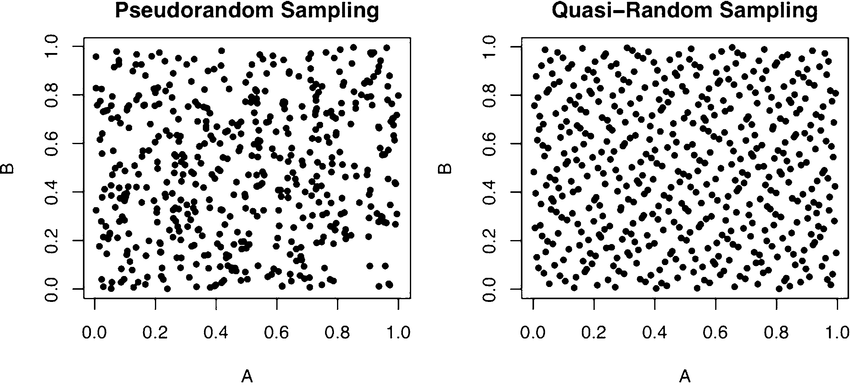
\includegraphics[width=0.7\textwidth]{pvsq.png} 
\end{frame}

\againframe{frame1}
\begin{frame}{QMC vs MC}
\begin{itemize}
\item Why use Quasi-Monte Carlo?
\item Generating lattices are not IID, some dependencies exists
\item Gives us faster convergence than pseudo random IID numbers.
\item Quasi Monte Carlo error almost $\mathcal{O}(\frac{1}{N})$ vs Monte Carlo is $\mathcal{O}(\frac{1}{\sqrt{N}})$.
\end{itemize}
\end{frame}

\begin{frame}{Results}%do these over various d
\begin{itemize}
\item Generated lattices from 6-8 times faster at least.
\item Function evaluations and averages computed on GPU.
\item Using Keister example we can get speed ups to about 10-12 times faster over CPU for high dimensions.
\item \[ \int_{\mathbb{R}^d}\cos(\|x\|)e^{-\|x\|^2} \textit{d}x\]
\end{itemize}
\end{frame}

\begin{frame}{Result Plot}
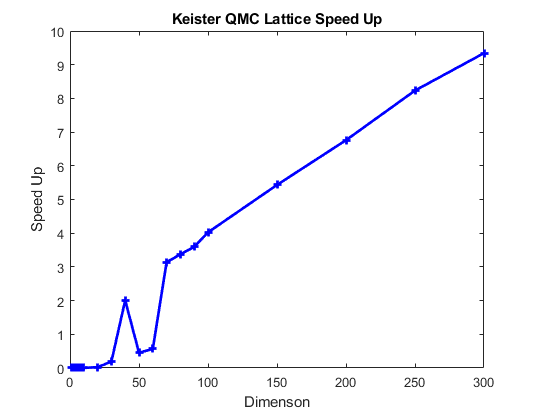
\includegraphics[width=\textwidth]{Keister_speed.png} 
\end{frame}

\begin{frame}{Shortfalls}
\begin{itemize}
\item We do not need FFT in parallel.
\item In GAIL GPU implementation of \textit{cublattice\_g} is good, but...
\item Complete integration into library is buggy.
\item GPU may not always be faster than CPU depending on problem
\end{itemize}
\end{frame}

\begin{frame}{GPU Hardware Bias}
\begin{itemize}
\item GPU computation is heavily hardware biased
\item Variety of products and manufactures
\item Measure dollars per performance speed up $\frac{\$}{\text{speed up}}$
\end{itemize}
\end{frame}

\begin{frame}{MC Examples of Hardware Bias}%Use M565 money example
\begin{itemize}
\item Easiest to see with a Pseudo-random number example
\item IID best for GPU do not have to rely on dependent samples
\item GTX 1050 (laptop GPU) MSRP \$400 vs GTX 1080 (Desktop GPU) MSRP \$700
\end{itemize}
\end{frame}

\begin{frame}{GPU Speed Up Cost}
\centering
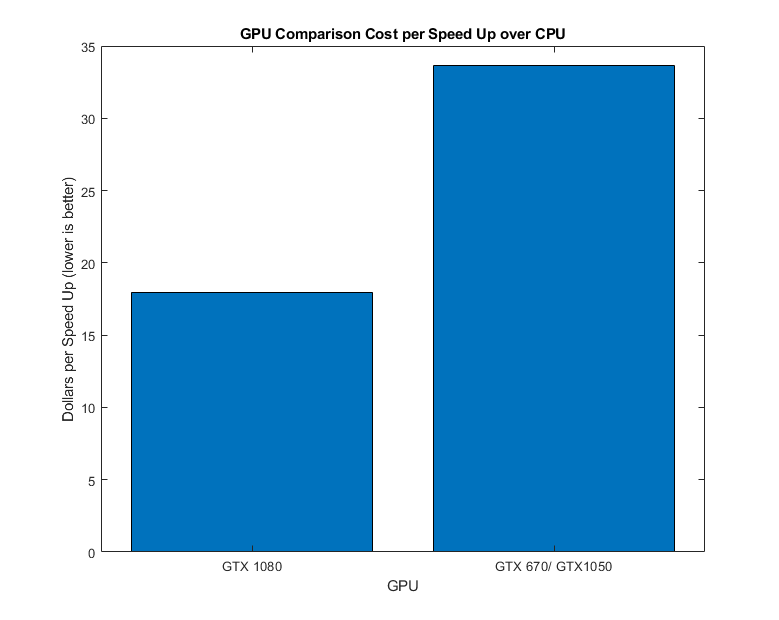
\includegraphics[width=0.85\textwidth]{gpuspeedup.png} 
\end{frame}

\begin{frame}{Further Work}
\begin{itemize}
\item Full integration of \textit{cublattice\_g} to work with entirety of GAIL
\item Extend GPU capabilities to IID Monte Carlo 
\item Other Quasi-Monte Carlo methods can sped up with GPU despite dependent sampling
\end{itemize}
\end{frame}

\begin{frame}{References}
\bibliographystyle{abbrv}
\bibliography{cs595_references}
\end{frame}
\end{document}